\documentclass[../main/NEMO_manual]{subfiles}

\begin{document}

\chapter{Space Domain (DOM)}
\label{chap:DOM}

% Missing things
% -    istate: description of the initial state   ==> this has to be put elsewhere..
%              perhaps in MISC ?  By the way the initialisation of T S and dynamics
%              should be put outside of DOM routine (better with TRC staff and off-line
%              tracers)
% - geo2ocean: how to switch from geographic to mesh coordinate
% -    domclo: closed sea and lakes....
%              management of closea sea area: specific to global cfg, both forced and coupled

\chaptertoc

\paragraph{Changes record} ~\\

{\footnotesize
  \begin{tabularx}{0.8\textwidth}{l||X|X}
    Release                                                                                 &
    Author(s)                                                                               &
    Modifications                                                                           \\
    \hline
    {\em 4.0                                                                              } &
    {\em Simon M\"{u}ller \& Andrew Coward \newline \newline
      Simona Flavoni and Tim Graham                                                       } &
    {\em Compatibility changes: many options moved to external domain configuration tools
      (see \autoref{apdx:DOMCFG}). \newline
      Updates                                                                             } \\
    {\em 3.6                                                                              } &
    {\em Rachid Benshila, Christian \'{E}th\'{e}, Pierre Mathiot and Gurvan Madec         } &
    {\em Updates                                                                          } \\
    {\em $\leq$ 3.4                                                                       } &
    {\em Gurvan Madec and S\'{e}bastien Masson                                            } &
    {\em First version                                                                    }
  \end{tabularx}
}

\clearpage

Having defined the continuous equations in \autoref{chap:MB} and
chosen a time discretisation \autoref{chap:TD},
we need to choose a grid for spatial discretisation and related numerical algorithms.
In the present chapter, we provide a general description of the staggered grid used in \NEMO,
and other relevant information about the DOM (DOMain) source code modules.

%% =================================================================================================
\section{Fundamentals of the discretisation}
\label{sec:DOM_basics}

%% =================================================================================================
\subsection{Arrangement of variables}
\label{subsec:DOM_cell}

\begin{figure}
  \centering
  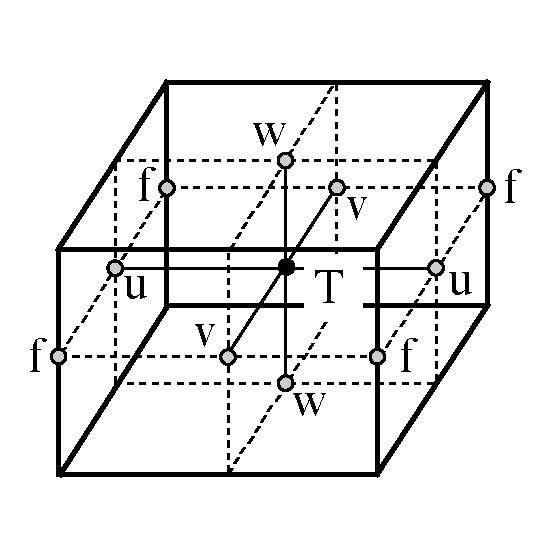
\includegraphics[width=0.33\textwidth]{DOM_cell}
  \caption[Arrangement of variables in the unit cell of space domain]{
    Arrangement of variables in the unit cell of space domain.
    $t$ indicates scalar points where
    temperature, salinity, density, pressure and horizontal divergence are defined.
    $(u,v,w)$ indicates vector points, and $f$ indicates vorticity points where
    both relative and planetary vorticities are defined.}
  \label{fig:DOM_cell}
\end{figure}

The numerical techniques used to solve the Primitive Equations in this model are based on
the traditional, centred second-order finite difference approximation.
Special attention has been given to the homogeneity of the solution in the three spatial directions.
The arrangement of variables is the same in all directions.
It consists of cells centred on scalar points ($t$, $S$, $p$, $\rho$) with
vector points $(u, v, w)$ defined in the centre of each face of the cells (\autoref{fig:DOM_cell}).
This is the generalisation to three dimensions of the well-known ``C'' grid in
Arakawa's classification \citep{mesinger.arakawa_bk76}.
The relative and planetary vorticity, $\zeta$ and $f$, are defined in the centre of each
vertical edge and the barotropic stream function $\psi$ is defined at horizontal points overlying
the $\zeta$ and $f$-points.

The ocean mesh (\ie\ the position of all the scalar and vector points) is defined by
the transformation that gives $(\lambda,\varphi,z)$ as a function of $(i,j,k)$.
The grid-points are located at integer or integer and a half value of $(i,j,k)$ as indicated on
\autoref{tab:DOM_cell}.
In all the following,
subscripts $u$, $v$, $w$, $f$, $uw$, $vw$ or $fw$ indicate the position of the grid-point where
the scale factors are defined.
Each scale factor is defined as the local analytical value provided by \autoref{eq:MB_scale_factors}.
As a result, the mesh on which partial derivatives $\pd[]{\lambda}$, $\pd[]{\varphi}$ and
$\pd[]{z}$ are evaluated is a uniform mesh with a grid size of unity.
Discrete partial derivatives are formulated by
the traditional, centred second order finite difference approximation while
the scale factors are chosen equal to their local analytical value.
An important point here is that the partial derivative of the scale factors must be evaluated by
centred finite difference approximation, not from their analytical expression.
This preserves the symmetry of the discrete set of equations and
therefore satisfies many of the continuous properties (see \autoref{apdx:INVARIANTS}).
A similar, related remark can be made about the domain size:
when needed, an area, volume, or the total ocean depth must be evaluated as
the product or sum of the relevant scale factors (see \autoref{eq:DOM_bar} in the next section).

\begin{table}
  \centering
  \begin{tabular}{|l|l|l|l|}
    \hline
    t   & $i      $ & $j      $ & $k      $ \\
    \hline
    u   & $i + 1/2$ & $j      $ & $k      $ \\
    \hline
    v   & $i      $ & $j + 1/2$ & $k      $ \\
    \hline
    w   & $i      $ & $j      $ & $k + 1/2$ \\
    \hline
    f   & $i + 1/2$ & $j + 1/2$ & $k      $ \\
    \hline
    uw  & $i + 1/2$ & $j      $ & $k + 1/2$ \\
    \hline
    vw  & $i      $ & $j + 1/2$ & $k + 1/2$ \\
    \hline
    fw  & $i + 1/2$ & $j + 1/2$ & $k + 1/2$ \\
    \hline
  \end{tabular}
  \caption[Location of grid-points]{
    Location of grid-points as a function of integer or
    integer and a half value of the column, line or level.
    This indexing is only used for the writing of the semi-discrete equations.
    In the code, the indexing uses integer values only and
    is positive downwards in the vertical with $k=1$ at the surface.
    (see \autoref{subsec:DOM_Num_Index})}
  \label{tab:DOM_cell}
\end{table}

Note that the definition of the scale factors
(\ie\ as the analytical first derivative of the transformation that
results in $(\lambda,\varphi,z)$ as a function of $(i,j,k)$)
is specific to the \NEMO\ model \citep{marti.madec.ea_JGR92}.
As an example, a scale factor in the $i$ direction is defined locally at a $t$-point,
whereas many other models on a C grid choose to define such a scale factor as
the distance between the $u$-points on each side of the $t$-point.
Relying on an analytical transformation has two advantages:
firstly, there is no ambiguity in the scale factors appearing in the discrete equations,
since they are first introduced in the continuous equations;
secondly, analytical transformations encourage good practice by
the definition of smoothly varying grids
(rather than allowing the user to set arbitrary jumps in thickness between adjacent layers)
\citep{treguier.dukowicz.ea_JGR96}.
An example of the effect of such a choice is shown in \autoref{fig:DOM_zgr_e3}.
\begin{figure}
  \centering
  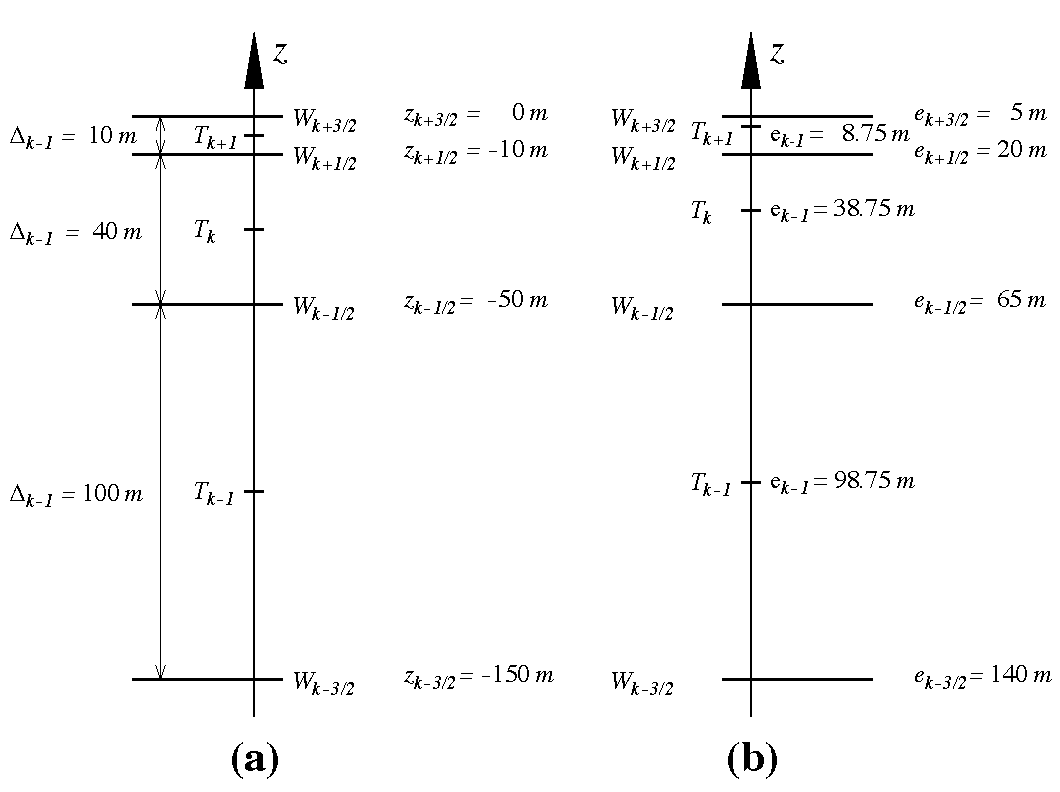
\includegraphics[width=0.5\textwidth]{DOM_zgr_e3}
  \caption[Comparison of grid-point position, vertical grid-size and scale factors]{
    Comparison of (a) traditional definitions of grid-point position and grid-size in the vertical,
    and (b) analytically derived grid-point position and scale factors.
    For both grids here, the same $w$-point depth has been chosen but
    in (a) the $t$-points are set half way between $w$-points while
    in (b) they are defined from an analytical function:
    $z(k) = 5 \, (k - 1/2)^3 - 45 \, (k - 1/2)^2 + 140 \, (k - 1/2) - 150$.
    Note the resulting difference between the value of the grid-size $\Delta_k$ and
    those of the scale factor $e_k$.}
  \label{fig:DOM_zgr_e3}
\end{figure}

%% =================================================================================================
\subsection{Discrete operators}
\label{subsec:DOM_operators}

Given the values of a variable $q$ at adjacent points,
the differencing and averaging operators at the midpoint between them are:
\begin{alignat*}{2}
  % \label{eq:DOM_di_mi}
  \delta_i [q]      &= &       &q (i + 1/2) - q (i - 1/2) \\
  \overline q^{\, i} &= &\big\{ &q (i + 1/2) + q (i - 1/2) \big\} / 2
\end{alignat*}

Similar operators are defined with respect to $i + 1/2$, $j$, $j + 1/2$, $k$, and $k + 1/2$.
Following \autoref{eq:MB_grad} and \autoref{eq:MB_lap},
the gradient of a variable $q$ defined at a $t$-point has
its three components defined at $u$-, $v$- and $w$-points while
its Laplacian is defined at the $t$-point.
These operators have the following discrete forms in the curvilinear $s$-coordinates system:
\begin{gather*}
  % \label{eq:DOM_grad}
  \nabla q \equiv   \frac{1}{e_{1u}} \delta_{i + 1/2} [q] \; \, \vect i
                  + \frac{1}{e_{2v}} \delta_{j + 1/2} [q] \; \, \vect j
                  + \frac{1}{e_{3w}} \delta_{k + 1/2} [q] \; \, \vect k \\
  % \label{eq:DOM_lap}
  \Delta q \equiv   \frac{1}{e_{1t} \, e_{2t} \, e_{3t}}
                    \; \lt[   \delta_i \lt( \frac{e_{2u} \, e_{3u}}{e_{1u}} \; \delta_{i + 1/2} [q] \rt)
                            + \delta_j \lt( \frac{e_{1v} \, e_{3v}}{e_{2v}} \; \delta_{j + 1/2} [q] \rt) \; \rt]
                  + \frac{1}{e_{3t}}
                              \delta_k \lt[ \frac{1              }{e_{3w}} \; \delta_{k + 1/2} [q] \rt]
\end{gather*}

Following \autoref{eq:MB_curl} and \autoref{eq:MB_div},
a vector $\vect A = (a_1,a_2,a_3)$ defined at vector points $(u,v,w)$ has
its three curl components defined at $vw$-, $uw$, and $f$-points, and
its divergence defined at $t$-points:
\begin{multline*}
% \label{eq:DOM_curl}
  \nabla \times \vect A \equiv   \frac{1}{e_{2v} \, e_{3vw}}
                                 \Big[   \delta_{j + 1/2} (e_{3w} \, a_3)
                                       - \delta_{k + 1/2} (e_{2v} \, a_2) \Big] \vect i \\
                               + \frac{1}{e_{2u} \, e_{3uw}}
                                 \Big[   \delta_{k + 1/2} (e_{1u} \, a_1)
                                       - \delta_{i + 1/2} (e_{3w} \, a_3) \Big] \vect j \\
                               + \frac{1}{e_{1f} \, e_{2f}}
                                 \Big[   \delta_{i + 1/2} (e_{2v} \, a_2)
                                       - \delta_{j + 1/2} (e_{1u} \, a_1) \Big] \vect k
\end{multline*}
\[
% \label{eq:DOM_div}
  \nabla \cdot \vect A \equiv   \frac{1}{e_{1t} \, e_{2t} \, e_{3t}}
                                \Big[ \delta_i (e_{2u} \, e_{3u} \, a_1) + \delta_j (e_{1v} \, e_{3v} \, a_2) \Big]
                              + \frac{1}{e_{3t}} \delta_k (a_3)
\]

The vertical average over the whole water column is denoted by an overbar and
is for a masked field $q$ (\ie\ a quantity that is equal to zero inside solid areas):
\begin{equation}
  \label{eq:DOM_bar}
  \bar q = \frac{1}{H} \int_{k^b}^{k^o} q \; e_{3q} \, dk \equiv \frac{1}{H_q} \sum \limits_k q \; e_{3q}
\end{equation}
where $H_q$  is the ocean depth, which is the masked sum of the vertical scale factors at $q$ points,
$k^b$ and $k^o$ are the bottom and surface $k$-indices,
and the symbol $\sum \limits_k$ refers to a summation over all grid points of the same type in
the direction indicated by the subscript (here $k$).

In continuous form, the following properties are satisfied:
\begin{gather}
  \label{eq:DOM_curl_grad}
  \nabla \times \nabla q = \vect 0 \\
  \label{eq:DOM_div_curl}
  \nabla \cdot (\nabla \times \vect A) = 0
\end{gather}

It is straightforward to demonstrate that these properties are verified locally in discrete form as
soon as the scalar $q$ is taken at $t$-points and the vector $\vect A$ has its components defined at
vector points $(u,v,w)$.

Let $a$ and $b$ be two fields defined on the mesh, with a value of zero inside continental areas.
It can be shown that the differencing operators ($\delta_i$, $\delta_j$ and
$\delta_k$) are skew-symmetric linear operators,
and further that the averaging operators ($\overline{\cdots}^{\, i}$, $\overline{\cdots}^{\, j}$ and
$\overline{\cdots}^{\, k}$) are symmetric linear operators, \ie
\begin{alignat}{5}
  \label{eq:DOM_di_adj}
  &\sum \limits_i a_i \; \delta_i [b]      &\equiv &- &&\sum \limits_i \delta      _{   i + 1/2} [a] &b_{i + 1/2} \\
  \label{eq:DOM_mi_adj}
  &\sum \limits_i a_i \; \overline b^{\, i} &\equiv &  &&\sum \limits_i \overline a ^{\, i + 1/2}     &b_{i + 1/2}
\end{alignat}

In other words,
the adjoint of the differencing and averaging operators are $\delta_i^* = \delta_{i + 1/2}$ and
$(\overline{\cdots}^{\, i})^* = \overline{\cdots}^{\, i + 1/2}$, respectively.
These two properties will be used extensively in the \autoref{apdx:INVARIANTS} to
demonstrate integral conservative properties of the discrete formulation chosen.

%% =================================================================================================
\subsection{Numerical indexing}
\label{subsec:DOM_Num_Index}

\begin{figure}
  \centering
  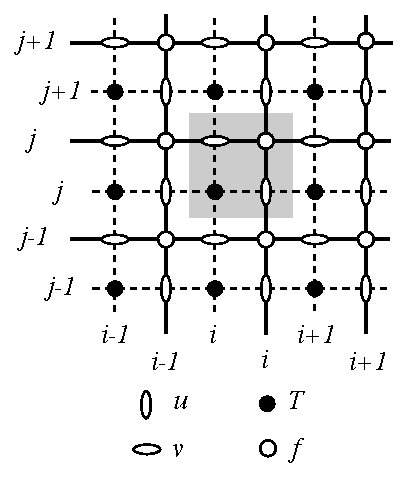
\includegraphics[width=0.33\textwidth]{DOM_index_hor}
  \caption[Horizontal integer indexing]{
    Horizontal integer indexing used in the \fortran\ code.
    The dashed area indicates the cell in which
    variables contained in arrays have the same $i$- and $j$-indices}
  \label{fig:DOM_index_hor}
\end{figure}

The array representation used in the \fortran\ code requires an integer indexing.
However, the analytical definition of the mesh (see \autoref{subsec:DOM_cell}) is associated with
the use of integer values for $t$-points only while
all the other points involve integer and a half values.
Therefore, a specific integer indexing has been defined for points other than $t$-points
(\ie\ velocity and vorticity grid-points).
Furthermore, the direction of the vertical indexing has been reversed and
the surface level set at $k = 1$.

%% =================================================================================================
\subsubsection{Horizontal indexing}
\label{subsec:DOM_Num_Index_hor}

The indexing in the horizontal plane has been chosen as shown in \autoref{fig:DOM_index_hor}.
For an increasing $i$ index ($j$ index),
the $t$-point and the eastward $u$-point (northward $v$-point) have the same index
(see the dashed area in \autoref{fig:DOM_index_hor}).
A $t$-point and its nearest north-east $f$-point have the same $i$-and $j$-indices.

%% =================================================================================================
\subsubsection{Vertical indexing}
\label{subsec:DOM_Num_Index_vertical}

In the vertical, the chosen indexing requires special attention since
the direction of the $k$-axis in the \fortran\ code is the reverse of
that used in the semi-discrete equations and given in \autoref{subsec:DOM_cell}.
The sea surface corresponds to the $w$-level $k = 1$,
which is the same index as the $t$-level just below (\autoref{fig:DOM_index_vert}).
The last $w$-level ($k = jpk$) either corresponds to or is below the ocean floor while
the last $t$-level is always outside the ocean domain (\autoref{fig:DOM_index_vert}).
Note that a $w$-point and the directly underlaying $t$-point have a common $k$ index
(\ie\ $t$-points and their nearest $w$-point neighbour in negative index direction),
in contrast to the indexing on the horizontal plane where
the $t$-point has the same index as the nearest velocity points in
the positive direction of the respective horizontal axis index
(compare the dashed area in \autoref{fig:DOM_index_hor} and \autoref{fig:DOM_index_vert}).
Since the scale factors are chosen to be strictly positive,
a \textit{minus sign} is included in the \fortran\ implementations of
\textit{all the vertical derivatives} of the discrete equations given in this manual in order to
accommodate the opposing vertical index directions in implementation and documentation.

\begin{figure}
  \centering
  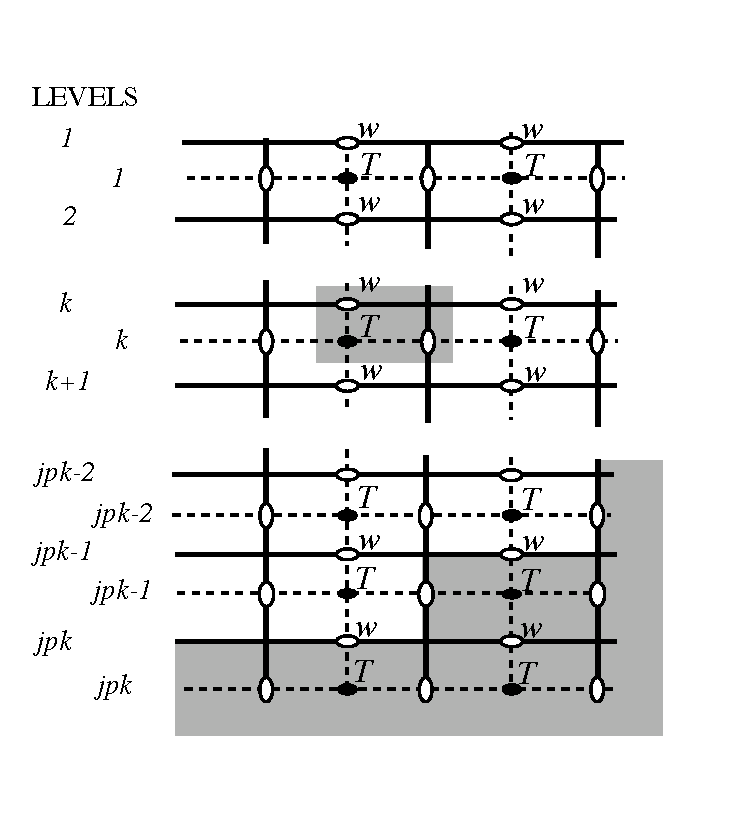
\includegraphics[width=0.33\textwidth]{DOM_index_vert}
  \caption[Vertical integer indexing]{
    Vertical integer indexing used in the \fortran\ code.
    Note that the $k$-axis is oriented downward.
    The dashed area indicates the cell in which
    variables contained in arrays have a common $k$-index.}
  \label{fig:DOM_index_vert}
\end{figure}

%% =================================================================================================
\section{Spatial domain configuration}
\label{subsec:DOM_config}

Two typical methods are available to specify the spatial domain configuration;
they can be selected using parameter \np{ln_read_cfg}{ln\_read\_cfg} parameter in
namelist \nam{cfg}{cfg}.

If \np{ln_read_cfg}{ln\_read\_cfg} is set to \forcode{.true.},
the domain-specific parameters and fields are read from a NetCDF input file,
whose name (without its .nc suffix) can be specified as
the value of the \np{cn_domcfg}{cn\_domcfg} parameter in namelist \nam{cfg}{cfg}.

If \np{ln_read_cfg}{ln\_read\_cfg} is set to \forcode{.false.},
the domain-specific parameters and fields can be provided (\eg\ analytically computed) by
subroutines \mdl{usrdef\_hgr} and \mdl{usrdef\_zgr}.
These subroutines can be supplied in the \path{MY_SRC} directory of the configuration,
and default versions that configure the spatial domain for the GYRE reference configuration are
present in the \path{./src/OCE/USR} directory.

In version 4.0 there are no longer any options for reading complex bathymetries and
performing a vertical discretisation at run-time.
Whilst it is occasionally convenient to have a common bathymetry file and, for example,
to run similar models with and without partial bottom boxes and/or sigma-coordinates,
supporting such choices leads to overly complex code.
Worse still is the difficulty of ensuring the model configurations intended to be identical are
indeed so when the model domain itself can be altered by runtime selections.
The code previously used to perform vertical discretisation has been incorporated into
an external tool (\path{./tools/DOMAINcfg}) which is briefly described in \autoref{apdx:DOMCFG}.

The next subsections summarise the parameter and fields related to
the configuration of the whole model domain.
These represent the minimum information that must be provided either via
the \np{cn_domcfg}{cn\_domcfg} file or
set by code inserted into user-supplied versions of the \texttt{usrdef\_*} subroutines.
The requirements are presented in three sections:
the domain size (\autoref{subsec:DOM_size}), the horizontal mesh (\autoref{subsec:DOM_hgr}),
and the vertical grid (\autoref{subsec:DOM_zgr}).

%% =================================================================================================
\subsection{Domain size}
\label{subsec:DOM_size}

The total size of the computational domain is set by the parameters \texttt{jpiglo}, \texttt{jpjglo} and
\texttt{jpkglo} for the $i$, $j$ and $k$ directions, respectively.
Note, that the variables \texttt{jpi} and \texttt{jpj} refer to
the size of each processor subdomain when the code is run in parallel using domain decomposition
(\key{mpp\_mpi} defined, see \autoref{sec:LBC_mpp}).

The name of the configuration is set through parameter \np{cn_cfg}{cn\_cfg},
and the nominal resolution through parameter \np{nn_cfg}{nn\_cfg}
(unless in the input file both of variables \texttt{ORCA} and \texttt{ORCA\_index} are present,
in which case \np{cn_cfg}{cn\_cfg} and \np{nn_cfg}{nn\_cfg} are set from these values accordingly).

The global lateral boundary condition type is selected from 8 options using parameters \texttt{l\_Iperio}, \texttt{l\_Jperio}, \texttt{l\_NFold} and \texttt{c\_NFtype}.
See \autoref{sec:LBC_jperio} for details on the available options and
the corresponding values for \texttt{l\_Iperio}, \texttt{l\_Jperio}, \texttt{l\_NFold} and \texttt{c\_NFtype}.

%% =================================================================================================
\subsection[Horizontal grid mesh (\textit{domhgr.F90}]{Horizontal grid mesh (\protect\mdl{domhgr})}
\label{subsec:DOM_hgr}

%% =================================================================================================
\subsubsection{Required fields}
\label{sec:DOM_hgr_fields}

The explicit specification of a range of mesh-related fields are required for
the definition of a configuration.
These include:

\begin{forlines}
integer   Ni0glo, NjOglo, jpkglo       /* global domain sizes (without MPI halos)                */
logical   l_Iperio, l_Jperio           /* lateral global domain b.c.: i- j-periodicity           */
logical   l_NFold                      /* lateral global domain b.c.: North Pole folding         */
char(1)   c_NFtype                     /*    type of North pole Folding: T or F point            */
real      glamt, glamu, glamv, glamf   /* geographic longitude (t,u,v and f points respectively) */
real      gphit, gphiu, gphiv, gphif   /* geographic latitude                                    */
real      e1t, e1u, e1v, e1f           /* horizontal scale factors                               */
real      e2t, e2u, e2v, e2f           /* horizontal scale factors                               */
\end{forlines}

The values of the geographic longitude and latitude arrays at indices $i,j$ correspond to
the analytical expressions of the longitude $\lambda$ and latitude $\varphi$ as a function of $(i,j)$,
evaluated at the values as specified in \autoref{tab:DOM_cell} for the respective grid-point position.
The calculation of the values of the horizontal scale factor arrays in general additionally involves
partial derivatives of $\lambda$ and $\varphi$ with respect to $i$ and $j$,
evaluated for the same arguments as $\lambda$ and $\varphi$.

%% =================================================================================================
\subsubsection{Optional fields}

\begin{forlines}
                        /* Optional:                                                 */
int    ORCA, ORCA_index /* configuration name, configuration resolution              */
double e1e2u, e1e2v     /* U and V surfaces (if grid size reduction in some straits) */
double ff_f, ff_t       /* Coriolis parameter (if not on the sphere)                 */
\end{forlines}

\NEMO\ can support the local reduction of key strait widths by
altering individual values of e2u or e1v at the appropriate locations.
This is particularly useful for locations such as Gibraltar or Indonesian Throughflow pinch-points
(see \autoref{sec:MISC_strait} for illustrated examples).
The key is to reduce the faces of $T$-cell
(\ie\ change the value of the horizontal scale factors at $u$- or $v$-point) but
not the volume of the cells.
Doing otherwise can lead to numerical instability issues.
In normal operation the surface areas are computed from $e1u * e2u$ and $e1v * e2v$ but
in cases where a gridsize reduction is required,
the unaltered surface areas at $u$ and $v$ grid points
(\texttt{e1e2u} and \texttt{e1e2v}, respectively) must be read or pre-computed in \mdl{usrdef\_hgr}.
If these arrays are present in the \np{cn_domcfg}{cn\_domcfg} file they are read and
the internal computation is suppressed.
Versions of \mdl{usrdef\_hgr} which set their own values of \texttt{e1e2u} and \texttt{e1e2v} should
set the surface-area computation flag:
\texttt{ie1e2u\_v} to a non-zero value to suppress their re-computation.

\smallskip
Similar logic applies to the other optional fields:
\texttt{ff\_f} and \texttt{ff\_t} which can be used to
provide the Coriolis parameter at F- and T-points respectively if the mesh is not on a sphere.
If present these fields will be read and used and
the normal calculation ($2 * \Omega * \sin(\varphi)$) suppressed.
Versions of \mdl{usrdef\_hgr} which set their own values of \texttt{ff\_f} and \texttt{ff\_t} should
set the Coriolis computation flag:
\texttt{iff} to a non-zero value to suppress their re-computation.

Note that longitudes, latitudes, and scale factors at $w$ points are exactly equal to
those of $t$ points, thus no specific arrays are defined at $w$ points.

%% =================================================================================================
\subsection[Vertical grid (\textit{domzgr.F90})]{Vertical grid (\protect\mdl{domzgr})}
\label{subsec:DOM_zgr}

\begin{listing}
  \nlst{namdom}
  \caption{\forcode{&namdom}}
  \label{lst:namdom}
\end{listing}

In the vertical, the model mesh is determined by four things:
\begin{enumerate}
\item the bathymetry given in meters;
\item the number of levels of the model (\texttt{jpk});
\item the analytical transformation $z(i,j,k)$ and the vertical scale factors
  (derivatives of the transformation); and
\item the masking system,
  \ie\ the number of wet model levels at each $(i,j)$ location of the horizontal grid.
\end{enumerate}

\begin{figure}
  \centering
  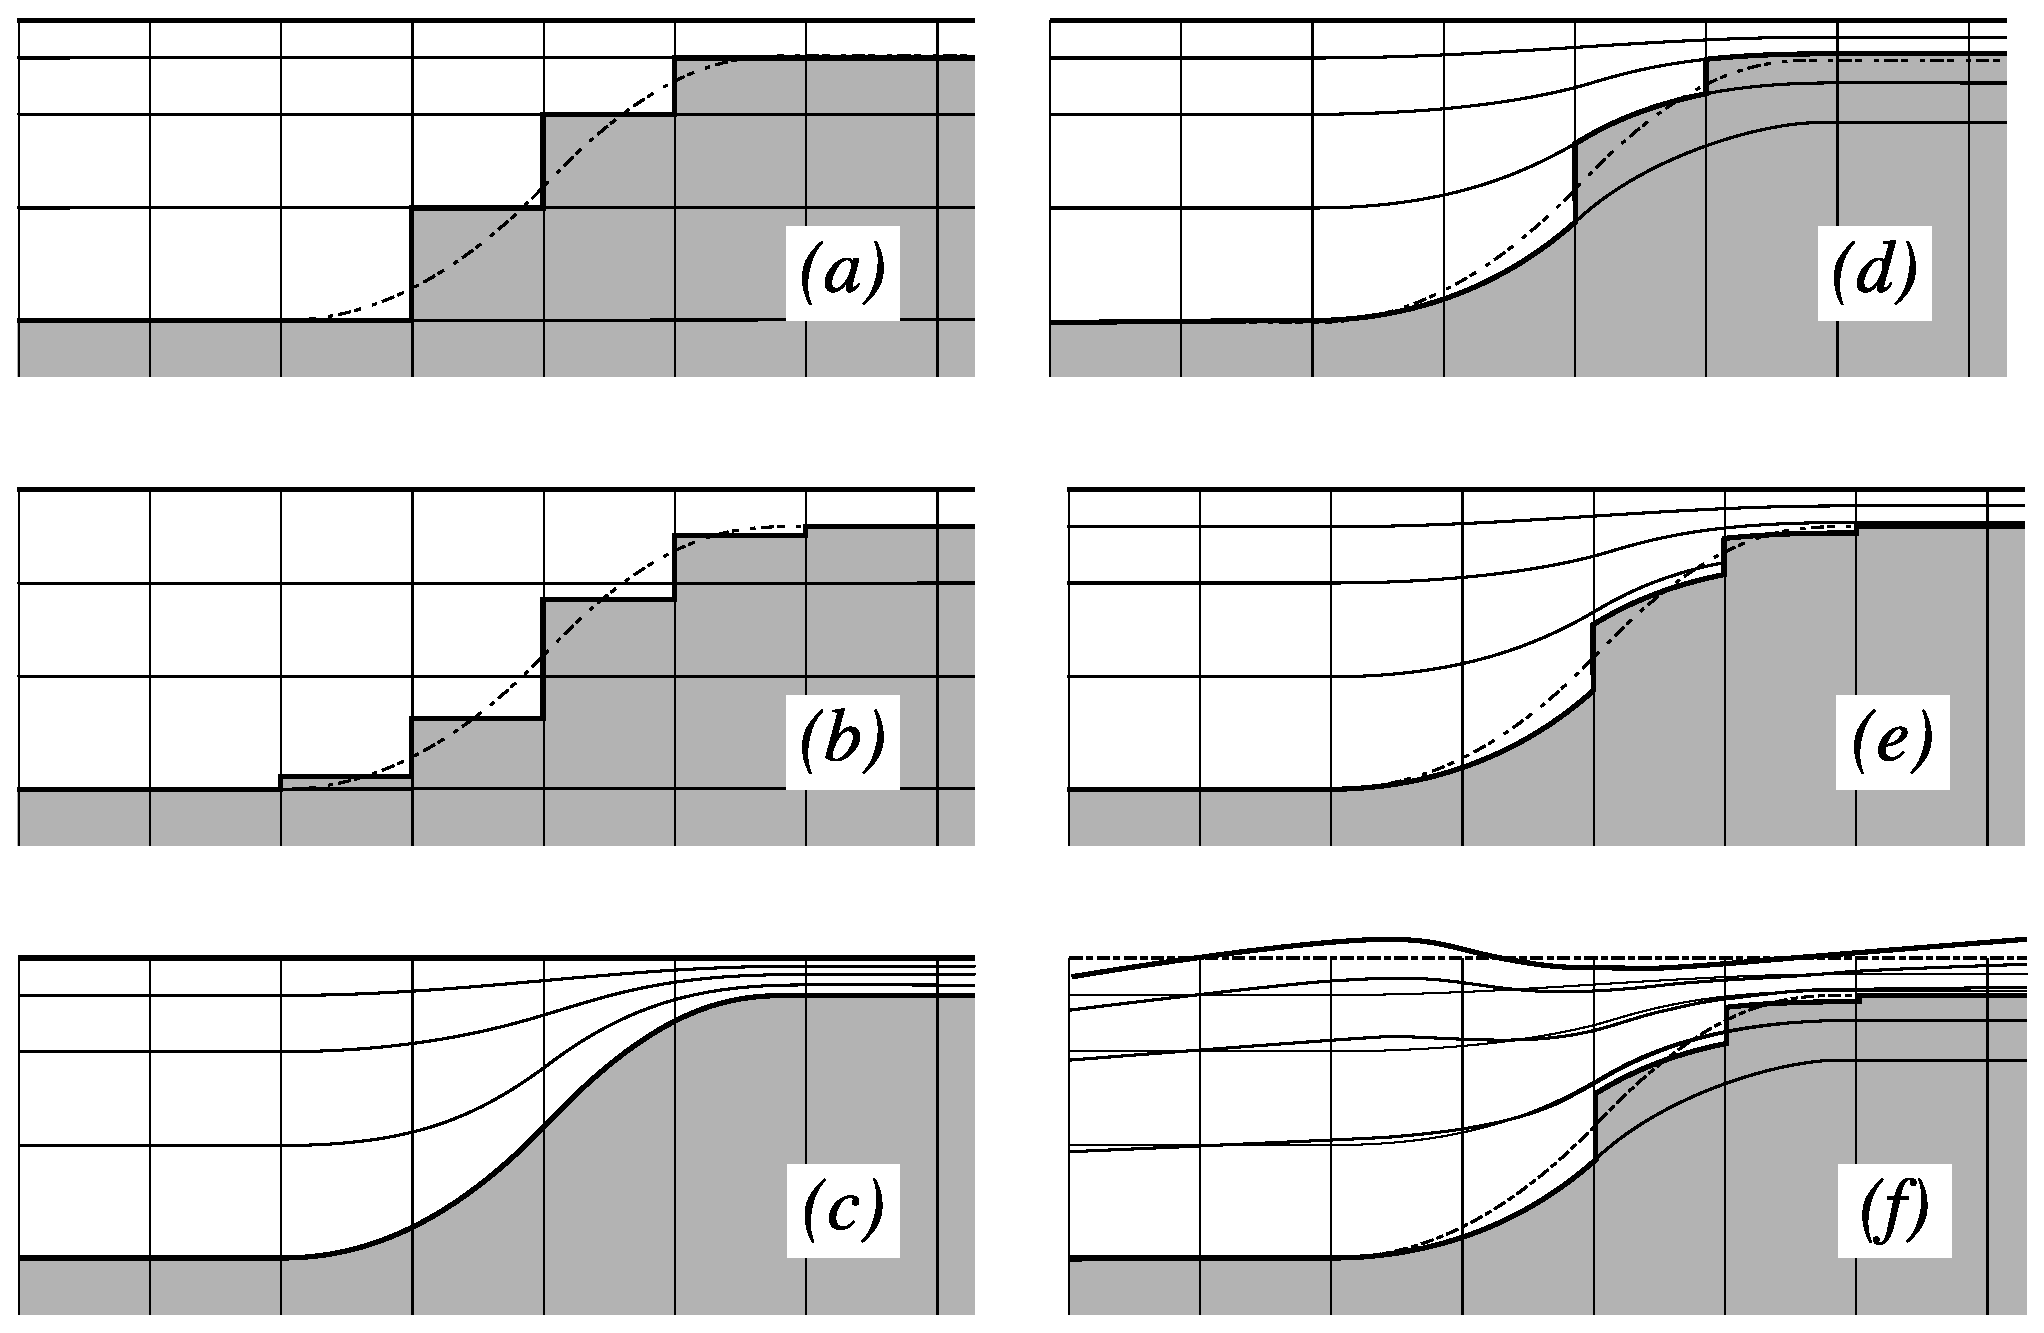
\includegraphics[width=0.5\textwidth]{DOM_z_zps_s_sps}
  \caption[Ocean bottom regarding coordinate systems ($z$, $s$ and hybrid $s-z$)]{
    The ocean bottom as seen by the model:
    \begin{enumerate*}[label=(\textit{\alph*})]
    \item $z$-coordinate with full step,
    \item $z$-coordinate with partial step,
    \item $s$-coordinate: terrain following representation,
    \item hybrid $s-z$ coordinate,
    \item hybrid $s-z$ coordinate with partial step, and
    \item same as (e) but in the non-linear free surface
      (\protect\np[=.false.]{ln_linssh}{ln\_linssh}).
  \end{enumerate*}
  Note that the non-linear free surface can be used with any of the 5 coordinates (a) to (e).}
  \label{fig:DOM_z_zps_s_sps}
\end{figure}

The choice of a vertical coordinate is made when setting up the configuration;
it is not intended to be an option which can be changed in the middle of an experiment.
The one exception to this statement being the choice of linear or non-linear free surface.
In v4.0 the linear free surface option is implemented as
a special case of the non-linear free surface.
This is computationally wasteful since it uses the structures for time-varying 3D metrics
for fields that (in the linear free surface case) are fixed.
However, the linear free-surface is rarely used and
implementing it this way means a single configuration file can support both options.

By default a non-linear free surface is used
(\np{ln_linssh}{ln\_linssh} set to \forcode{=.false.} in \nam{dom}{dom}):
the coordinate follow the time-variation of the free surface so that
the transformation is time dependent: $z(i,j,k,t)$ (\eg\ \autoref{fig:DOM_z_zps_s_sps}f).
When a linear free surface is assumed
(\np{ln_linssh}{ln\_linssh} set to \forcode{=.true.} in \nam{dom}{dom}),
the vertical coordinates are fixed in time, but
the seawater can move up and down across the $z_0$ surface
(in other words, the top of the ocean in not a rigid lid).

Note that settings:
\np{ln_zco}{ln\_zco}, \np{ln_zps}{ln\_zps}, \np{ln_sco}{ln\_sco} and \np{ln_isfcav}{ln\_isfcav}
mentioned in the following sections appear to be namelist options but
they are no longer truly namelist options for \NEMO.
Their value is written to and read from the domain configuration file and
they should be treated as fixed parameters for a particular configuration.
They are namelist options for the \texttt{DOMAINcfg} tool that can be used to
build the configuration file and serve both to provide a record of the choices made whilst
building the configuration and to trigger appropriate code blocks within \NEMO.
These values should not be altered in the \np{cn_domcfg}{cn\_domcfg} file.

\medskip
The decision on these choices must be made when the \np{cn_domcfg}{cn\_domcfg} file is constructed.
Three main choices are offered (\autoref{fig:DOM_z_zps_s_sps}a-c):

\begin{itemize}
\item $z$-coordinate with full step bathymetry (\np[=.true.]{ln_zco}{ln\_zco}),
\item $z$-coordinate with partial step ($zps$) bathymetry (\np[=.true.]{ln_zps}{ln\_zps}),
\item Generalized, $s$-coordinate (\np[=.true.]{ln_sco}{ln\_sco}).
\end{itemize}

Additionally, hybrid combinations of the three main coordinates are available:
$s-z$ or $s-zps$ coordinate (\autoref{fig:DOM_z_zps_s_sps}d and \autoref{fig:DOM_z_zps_s_sps}e).

A further choice related to vertical coordinate concerns
the presence (or not) of ocean cavities beneath ice shelves within the model domain.
A setting of \np{ln_isfcav}{ln\_isfcav} as \forcode{.true.} indicates that
the domain contains ocean cavities,
otherwise the top, wet layer of the ocean will always be at the ocean surface.
This option is currently only available for $z$- or $zps$-coordinates.
In the latter case, partial steps are also applied at the ocean/ice shelf interface.

Within the model,
the arrays describing the grid point depths and vertical scale factors are
three set of three dimensional arrays $(i,j,k)$ defined at
\textit{before}, \textit{now} and \textit{after} time step.
The time at which they are defined is indicated by a suffix: $\_b$, $\_n$, or $\_a$, respectively.
They are updated at each model time step.
The initial fixed reference coordinate system is held in variable names with a $\_0$ suffix.
When the linear free surface option is used (\np[=.true.]{ln_linssh}{ln\_linssh}),
\textit{before}, \textit{now} and \textit{after} arrays are initially set to
their reference counterpart and remain fixed.

%% =================================================================================================
\subsubsection{Required fields}
\label{sec:DOM_zgr_fields}

The explicit specification of a range of fields related to the vertical grid are required for
the definition of a configuration.
These include:

\begin{forlines}
int    ln_zco, ln_zps, ln_sco            /* flags for z-coord, z-coord with partial steps and s-coord    */
int    ln_isfcav                         /* flag  for ice shelf cavities                                 */
double e3t_1d, e3w_1d                    /* reference vertical scale factors at T and W points           */
double e3t_0, e3u_0, e3v_0, e3f_0, e3w_0 /* vertical scale factors 3D coordinate at T,U,V,F and W points */
double e3uw_0, e3vw_0                    /* vertical scale factors 3D coordinate at UW and VW points     */
int    bottom_level, top_level           /* last wet T-points, 1st wet T-points (for ice shelf cavities) */
                                         /* For reference:                                               */
float  bathy_metry                       /* bathymetry used in setting top and bottom levels             */
\end{forlines}

This set of vertical metrics is sufficient to describe the initial depth and thickness of
every gridcell in the model regardless of the choice of vertical coordinate.
With constant z-levels, e3 metrics will be uniform across each horizontal level.
In the partial step case each e3 at the \texttt{bottom\_level}
(and, possibly, \texttt{top\_level} if ice cavities are present)
may vary from its horizontal neighbours.
And, in s-coordinates, variations can occur throughout the water column.
With the non-linear free-surface, all the coordinates behave more like the s-coordinate in that
variations occur throughout the water column with displacements related to the sea surface height.
These variations are typically much smaller than those arising from bottom fitted coordinates.
The values for vertical metrics supplied in the domain configuration file can be considered as
those arising from a flat sea surface with zero elevation.

The \texttt{bottom\_level} and \texttt{top\_level} 2D arrays define
the \texttt{bottom\_level} and top wet levels in each grid column.
Without ice cavities, \texttt{top\_level} is essentially a land mask (0 on land; 1 everywhere else).
With ice cavities, \texttt{top\_level} determines the first wet point below the overlying ice shelf.

%% =================================================================================================
\subsubsection{Level bathymetry and mask}
\label{subsec:DOM_msk}

From \texttt{top\_level} and \texttt{bottom\_level} fields, the mask fields are defined as follows:
\begin{align*}
  tmask(i,j,k) &=
  \begin{cases}
    0 &\text{if $                             k <    top\_level(i,j)$} \\
    1 &\text{if $     bottom\_level(i,j) \leq k \leq top\_level(i,j)$} \\
    0 &\text{if $k >  bottom\_level(i,j)                            $}
  \end{cases} \\
  umask(i,j,k) &= tmask(i,j,k) * tmask(i + 1,j,    k) \\
  vmask(i,j,k) &= tmask(i,j,k) * tmask(i    ,j + 1,k) \\
  fmask(i,j,k) &= tmask(i,j,k) * tmask(i + 1,j,    k) * tmask(i,j,k) * tmask(i + 1,j,    k) \\
  wmask(i,j,k) &= tmask(i,j,k) * tmask(i    ,j,k - 1) \\
  \text{with~} wmask(i,j,1) &= tmask(i,j,1)
\end{align*}

Note that, without ice shelves cavities,
masks at $t-$ and $w-$points are identical with the numerical indexing used
(\autoref{subsec:DOM_Num_Index}).
Nevertheless,
$wmask$ are required with ocean cavities to deal with the top boundary (ice shelf/ocean interface)
exactly in the same way as for the bottom boundary.

%% The specification of closed lateral boundaries requires that at least
%% the first and last rows and columns of the \textit{mbathy} array are set to zero.
%% In the particular case of an east-west cyclical boundary condition, \textit{mbathy} has its last column equal to
%% the second one and its first column equal to the last but one (and so too the mask arrays)
%% (see \autoref{fig:LBC_jperio}).

%        Closed seas
%% =================================================================================================
\subsection{Closed seas}
\label{subsec:DOM_closea}

When a global ocean is coupled to an atmospheric model it is better to
represent all large water bodies (\eg\ Great Lakes, Caspian sea, \dots) even if
the model resolution does not allow their communication with the rest of the ocean.
This is unnecessary when the ocean is forced by fixed atmospheric conditions,
so these seas can be removed from the ocean domain.
The user has the option to
set the bathymetry in closed seas to zero (see \autoref{sec:MISC_closea}) and to
optionally decide on the fate of any freshwater imbalance over the area.
The options are explained in \autoref{sec:MISC_closea} but
it should be noted here that a successful use of these options requires
appropriate mask fields to be present in the domain configuration file.

%% =================================================================================================
\subsection{Output grid files}
\label{subsec:DOM_meshmask}

Most of the arrays relating to a particular ocean model configuration discussed in this chapter
(grid-point position, scale factors) can be saved in a file if
namelist parameter \np{ln_write_cfg}{ln\_write\_cfg} (namelist \nam{cfg}{cfg}) is set to
\forcode{.true.};
the output filename is set through parameter \np{cn_domcfg_out}{cn\_domcfg\_out}.
This is only really useful if
the fields are computed in subroutines \mdl{usrdef\_hgr} or \mdl{usrdef\_zgr} and
checking or confirmation is required.

Alternatively, all the arrays relating to a particular ocean model configuration
(grid-point position, scale factors, depths and masks) can be saved in
a file called \texttt{mesh\_mask} if
namelist parameter \np{ln_meshmask}{ln\_meshmask} (namelist \nam{dom}{dom}) is set to
\forcode{.true.}.
This file contains additional fields that can be useful for post-processing applications.

%% =================================================================================================
\section[Initial state (\textit{istate.F90} and \textit{dtatsd.F90})]{Initial state (\protect\mdl{istate} and \protect\mdl{dtatsd})}
\label{sec:DOM_DTA_tsd}

\begin{listing}
  \nlst{namtsd}
  \caption{\forcode{&namtsd}}
  \label{lst:namtsd}
\end{listing}

Basic initial state options are defined in \nam{tsd}{tsd}.
By default, the ocean starts from rest (the velocity field is set to zero) and
the initialization of temperature and salinity fields is controlled through the \np{ln_tsd_init}{ln\_tsd\_init} namelist parameter.

\begin{description}
\item [{\np[=.true.]{ln_tsd_init}{ln\_tsd\_init}}] Use T and S input files that can be given on
  the model grid itself or on their native input data grids.
  In the latter case,
  the data will be interpolated on-the-fly both in the horizontal and the vertical to the model grid
  (see \autoref{subsec:SBC_iof}).
  The information relating to the input files are specified in
  the \np{sn_tem}{sn\_tem} and \np{sn_sal}{sn\_sal} structures.
  The computation is done in the \mdl{dtatsd} module.
\item [{\np[=.false.]{ln_tsd_init}{ln\_tsd\_init}}] Initial values for T and S are set via
  a user supplied \rou{usr\_def\_istate} routine contained in \mdl{userdef\_istate}.
  The default version sets horizontally uniform T and profiles as used in the GYRE configuration
  (see \autoref{sec:CFGS_gyre}).
\end{description}

\subinc{%% =================================================================================================
%% Backmatter
%% =================================================================================================

%% Bibliography
%% =================================================================================================

\phantomsection
\addcontentsline{toc}{chapter}{Bibliography}
\lohead{Bibliography}
\rehead{Bibliography}
\bibliography{../main/bibliography}

\clearpage

%% Indices
%% =================================================================================================

\phantomsection
\addcontentsline{toc}{chapter}{Indices}
\lohead{Indices}
\rehead{Indices}
\printindex[blocks]
\printindex[keys]
\printindex[modules]
\printindex[parameters]
\printindex[subroutines]

\clearpage

%% Glossary
%% =================================================================================================

%\phantomsection
%\addcontentsline{toc}{chapter}{Glossary}
%\lohead{Glossary}\rehead{Glossary}
%\printglossaries
}

\end{document}
